\documentclass[11pt,letterpaper]{article}
\usepackage[top=3cm, bottom=2cm, left=2cm, right=2cm, columnsep=20pt]{geometry}
\usepackage{pdfpages}
\usepackage{graphicx}
\usepackage{etoolbox}
\apptocmd{\sloppy}{\hbadness 10000\relax}{}{}
% \usepackage[numbers]{natbib}
\usepackage[T1]{fontenc}
\usepackage{ragged2e}
\usepackage[french]{babel}
\usepackage{listings}
\usepackage{color}
\usepackage{soul}
\usepackage[utf8]{inputenc}
\usepackage[export]{adjustbox}
\usepackage{caption}
\usepackage{amsmath}
\usepackage{amssymb}
\usepackage{float}
\usepackage{csquotes}
\usepackage{fancyhdr}
\usepackage{wallpaper}
\usepackage{siunitx}
\usepackage[indent]{parskip}
\usepackage{textcomp}
\usepackage{gensymb}
\usepackage{multirow}
\usepackage[hidelinks]{hyperref}
\usepackage{abstract}
\usepackage{braket}
\renewcommand{\abstractnamefont}{\normalfont\bfseries}
\renewcommand{\abstracttextfont}{\normalfont\itshape}
\usepackage{titlesec}
\titleformat{\section}{\large\bfseries}{\thesection}{1em}{}
\titleformat{\subsection}{\normalsize\bfseries}{\thesubsection}{1em}{}
\titleformat{\subsubsection}{\normalsize\bfseries}{\thesubsubsection}{1em}{}

\usepackage{xcolor}
\definecolor{codegreen}{rgb}{0,0.6,0}
\definecolor{codegray}{rgb}{0.5,0.5,0.5}
\definecolor{codepurple}{rgb}{0.58,0,0.82}
\definecolor{backcolour}{rgb}{0.95,0.95,0.92}
\lstdefinestyle{mystyle}{
    backgroundcolor=\color{backcolour},   
    commentstyle=\color{codegreen},
    keywordstyle=\color{magenta},
    numberstyle=\tiny\color{codegray},
    stringstyle=\color{codepurple},
    basicstyle=\ttfamily\footnotesize,
    breakatwhitespace=false,         
    breaklines=true,                 
    captionpos=b,                    
    keepspaces=true,                 
    numbers=left,                    
    numbersep=5pt,                  
    showspaces=false,                
    showstringspaces=false,
    showtabs=false,                  
    tabsize=2
}
\lstset{style=mystyle}

\usepackage[most]{tcolorbox}
\newtcolorbox{note}[1][]{
  enhanced jigsaw,
  borderline west={2pt}{0pt}{black},
  sharp corners,
  boxrule=0pt, 
  fonttitle={\large\bfseries},
  coltitle={black},
  title={Note:\ },
  attach title to upper,
  #1
}

%----------------------------------------------------

\newcommand*{\Coord}[2]{% 
    \begin{pmatrix} 
      #1\\ 
      #2 
    \end{pmatrix}}

\setlength{\parindent}{0pt}
\DeclareCaptionLabelFormat{mycaptionlabel}{#1 #2}
\captionsetup[figure]{labelsep=colon}
\captionsetup{labelformat=mycaptionlabel}
\captionsetup[figure]{name={Figure }}
\newcommand{\inlinecode}{\normalfont\texttt}
\usepackage{enumitem}
\setlist[itemize]{label=\textbullet}

\begin{document}
\begin{titlepage}
\center

\begin{figure}
    \ThisULCornerWallPaper{.4}{Polytechnique_signature-RGB-gauche_FR.png}
\end{figure}
\vspace*{2 cm}

\textsc{\Large \textbf{PHS2223 --} Introduction à l'optique moderne}\\[0.5cm]
\large{\textbf{Équipe : 04}}\\[1.5cm]

\rule{\linewidth}{0.5mm} \\[0.5cm]
\Large{\textbf{Expérience 3}} \\[0.2cm]
\text{Mesure de polarisation}\\
\rule{\linewidth}{0.2mm} \\[2.3cm]

\large{\textbf{Présenté à}\\
  Guillaume Sheehy\\
  Esmat Zamani\\[2.5cm]
  \textbf{Par :}\\
  Émile \textbf{Guertin-Picard} (2208363)\\
  Laura-Li \textbf{Gilbert} (2204234)\\
  Tom \textbf{Dessauvages} (2133573)\\[3cm]}

\large{\today\\
Département de Génie Physique\\
Polytechnique Montréal\\}

\end{titlepage}

%----------------------------------------------------

\tableofcontents
\pagenumbering{roman}
\newpage

\pagestyle{fancy}
\setlength{\headheight}{14pt}
\renewcommand{\headrulewidth}{0pt}
\fancyfoot[R]{\thepage}

\pagestyle{fancy}
\fancyhf{}
\renewcommand{\headrulewidth}{1pt}
\fancyhead[L]{\textbf{PHS2223}}
\fancyhead[C]{Mesure de polarisation}
\fancyhead[R]{\today}
\fancyfoot[R]{\thepage}

\pagenumbering{arabic}
\setcounter{page}{1}

%----------------------------------------------------

\section{Résultats}\label{res}

Suite à la prise de données au laboratoire, il est possible de comparer les valeurs de
coefficients de transmission obtenus aux hypothèses émises pour les mesures à deux et trois polariseurs.
En reprenant la courbe proportionnelle à $\cos^{2}\left( \theta \right)$ pour le montage de
deux polariseurs, la figure \ref{2pol} montre les valeurs obtenues, qui suivent très bien la
tendance prédite.

\begin{figure}[H]
  \centering
  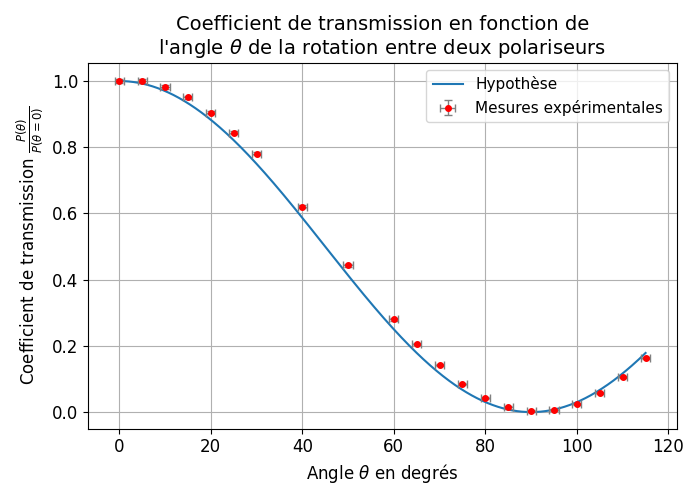
\includegraphics[scale=0.7]{viz_deux_pol.png}
  \caption{Résultats de la prise de mesure superposée à la prédiction de l'hypothèse pour la 
  mesure à deux polariseurs.}
  \label{2pol}
\end{figure}

De même pour le montage à trois polariseurs, la figure \ref{3pol} montre les valeurs de coefficient
de transmission expérimentales, qui suivent aussi bien la courbe proportionnelle à 
$\cos^{4}\left( \theta \right)$ émise par l'hypothèse.

\begin{figure}[H]
  \centering
  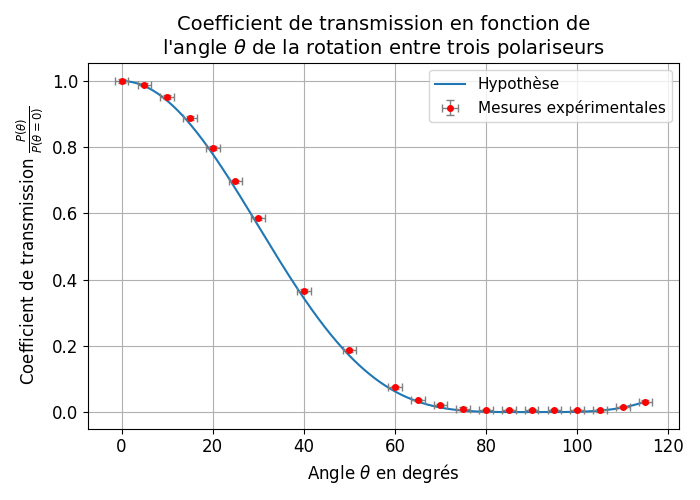
\includegraphics[scale=0.7]{viz_trois_pol.png}
  \caption{Résultats de la prise de mesure superposée à la prédiction de l'hypothèse pour la 
  mesure à trois polariseurs.}
  \label{3pol}
\end{figure}

Les incertitudes présentées avec les barres d'erreurs dans les graphiques ont été trouvées comme suit.
Pour les incertitudes sur l'angle $\theta$, la valeur est tout simplement la moitié de la plus petite
graduation sur les cadrans gradués, multiplié par le nombre de cadrans utilisés. Ainsi, pour les
mesures à deux polariseurs, comme la plus petite graduation était de $1\degree$, l'incertitude 
$\Delta\theta$  sur l'angle est aussi de $1\degree$. Pour trois polariseurs, $\Delta\theta = 1.5\degree$.
Quant aux incertitudes au compteur de puissance, elles sont trouvées par la plus petite valeur lisible au
compteur de puissance, soit $0.001$ mW. Les incertitudes pour les angles dans les barres d'erreurs des graphiques sont données 
directement par $\Delta\theta$. Les incertitudes sur les coefficients de transmission sont plus complexes
à obtenir. Leur calcul est détaillé à la section \ref{inc}. Danc ces calculs, en remplaçant par les valeurs numériques obtenues 
lors des expériences, il est possible d'estimer l'erreur sur les ordonnées en posant une borne supérieure 
sur la valeur qu'elle peut prendre :

\begin{align*}
  \text{Deux polariseurs : }\Delta C &\leq 0.005\\ 
  \text{Trois polariseurs : }\Delta C &\leq 0.008
\end{align*}

Les erreurs relatives maximales, étant donné que les coefficients à l'angle $\theta= 0$ sont donc de 0.5\% et de 0.8\% pour deux et trois polariseurs, ce qui est faible et signe d'un résultat avec une bonne exactitude.

\section{Discussion}

Cette section est consacrée à l'analyse des résultats obtenus et à la discussion sur les concepts employés
lors de ce laboratoire.

\subsection{Estimation des erreurs}\label{inc}

Pour les incertitudes sur les coefficients de transmission $C$, le point de départ est la formule du coefficient :

\begin{equation}
  C = \frac{P}{P_{0}},
\end{equation}

où $P$ est la puissance mesurée à un certain angle $\theta$ et $P_{0}$ est $P\left( \theta= 0 \right)$.
La propagation d'erreur pour une division de la sorte permet de calculer l'incertitude sur $C$ pour un
certain $P$ \textcolor{red}{source A} :

\begin{equation}\label{deltac}
  \Delta C = C\sqrt{\left( \frac{\Delta P}{P} \right)^{2} + \left( \frac{\Delta P_{0}}{P_{0}} \right)^{2}},
\end{equation}

où $\Delta P$ et $\Delta P_{0}$ sont les incertitudes correspondant à la plus petite valeur lisible au
compteur de puissance, tel que discuté plus tôt. Selon le modèle mathématique de 
l'erreur $\Delta C$ et selon les données expérimentales, il est possible de voir que l'erreur maximale 
est en $\theta= 0$ où $C$ est maximal. Ainsi, les bornes sur l'erreur de la section \ref{res} proviennent
de l'insertion de $C\left( \theta= 0 \right)$ dans (\ref{deltac}) pour obtenir les valeurs numériques pour
les cas à deux et trois polariseurs.

% Source A : https://chem.libretexts.org/Bookshelves/Analytical_Chemistry/Supplemental_Modules_(Analytical_Chemistry)/Quantifying_Nature/Significant_Digits/Propagation_of_Error


\subsection{Analyse des causes d'erreurs}

 Les erreurs présentées dans la partie 1.1 du rapport sont principalement dues aux imperfections des systèmes physiques utilisés, notamment lors du calcul de l'intensité après avoir placé le premier polarisateur qui aurait été, dans un cas idéal, divisée par deux peu importe la direction du polarisateur. Les valeurs obtenues, dans ce cas, sont plutôt de l'ordre de 0.32 fois la valeur initiale. Cette différence s'explique principalement grâce aux imperfections des filtres polarisateurs utilisés, 0.32 est une valeur approximative, variant elle-même d'un filtre à l'autre. Elle doit aussi être due à la lumière présente dans la pièce, dont l'impact parait néanmoins négligeable aux vues des valeurs de minimum mesurées qui avoisinaient les 0.001 mW. De plus, le réseau lampe/lentille positionné en entrée du montage devait produire, dans un cas idéal, un faisceau collimaté jusqu'à la seconde lentille. Lors de la mise en pratique, ce faisceau avait une forme conique principalement due aux imperfections de la lampe utilisée dont les rayons divergeaient.

\subsection{Lien avec le formalisme de Jones}\label{jonesjones}

En optique, la méthode des matrices permet de décrire l'impact d'un système physique composé de lentilles, miroirs, filtres, 
polarisateurs, etc. sur un faisceau le traversant, en fonction de sa position vis-à-vis de l'axe optique, et de son angle 
d'entrée. Un tel système s'exprime mathématiquement par une sorte de fonction de transfert, par exemple : 

\begin{equation}
    y_{out} = Ay_{in},
\end{equation}

Où $y$  représente les rayons d'entrée et de sortie, et $A$ représente le système physique. Dans le formalisme optique, $A$ 
prend la forme d'une matrice et $y$ d'un vecteur, exactement comme en mécanique quantique. Si on considère $\ket{y}$ comme 
étant l'état du faisceau, la fonction de transfert $A$ du système optique peut être interprétée comme un opérateur, tel que : 

\begin{equation}
    \ket{y_{out}} = \hat{A}\ket{y_{in}}.
\end{equation}

Ainsi, pour une polarisation planaire, le modèle de Jones considère une base $\{$$\ket{\hat{x}}$, $\ket{\hat{y}}$$\}$ telle 
que tout état de polarisation puisse être exprimé comme :

\begin{equation}
    \ket{y} = a\ket{\hat{x}} + b\ket{\hat{y}} = a\Coord{1}{0} + b\Coord{0}{1},
\end{equation}

Où $a^2 + b^2 = 1$ et les kets de la base sont deux vecteurs orthonormaux. Les photons, étant des particules de spin 1 pour 
lesquels l'état 0 est inaccessible, la base géométrique $\{$$\ket{\hat{x}}$, $\ket{\hat{y}}$$\}$ fait un lien direct avec 
la notion de spin quantique au niveau de son formalisme. Le détail de ce formalisme est présenté dans le procédurier du 
laboratoire \textcolor{red}{procedurier}. Pour le système de polaristeur utilisé lors du laboratoire, il serait possible, par
exemple, d'avoir  : 

\begin{equation*}
    \hat{A} = \hat{P_3}\hat{P_2}\hat{P_1} = \frac{1}{2}\Coord{1 \quad \pm 1}{\pm 1 \quad 1}\Coord{0 \quad 0}{0 \quad 1}\Coord{1 \quad 0}{0 \quad 0},
\end{equation*}

Où $\hat{P_1}$ serait alors un polariseur horizontal, $\hat{P_2}$ vertical et $\hat{P_3}$ diagonal à $\pm$45°. Tel qu'attendu, le produit matriciel donne 0 : une
lumière polarisée horizontalement se retrouve entièrement bloquée par un polarisateur vertical. L'application de $\hat{A}$ sur un état de la base, donc à une polarisation linéraire, retourne un vecteur nul. Cela illustre que le traitement
des états par kets et des éléments d'un système par opérateur est identique pour le formalisme quantique que pour celui de Jones, entre autres de par le fait que la base présentée pour le modèle de Jones est pratiquement indistinguable à la base des particules de spin $\frac{1}{2}$. Tel que spécifié, même si les photons sont de spin 1, comme l'état 0 est inaccessible, sa base contient aussi seulement deux éléments.

\subsection{Question 1}
Pour fabriquer un filtre à transmission ajustable, il est possible d'utiliser le même principe que celui réalisé dans cette expérience. En d'autres termnes, en utilisant deux polariseurs linéaires, placés en série avec un angle variable entre leurs axes de polarisation, la transmission devient dépendante de la valeur de l'angle. Ainsi, un filtre de transmission ajustable est créé. Cette méthode fonctionne pour tous les types de faisceaux. Cependant, selon le type de celui-ci, un différent nombre de filtre est nécessaire. Si le faisceau n'est pas polarisé, deux filtres doivent être utilisés alors que, si le faisceau est polarisé, un seul filtre est nécessaire.

\subsection{Question 2}
Pour provoquer une rotation de l'état de polarisation de 90$^\circ$, il est possible d'utiliser une série de polariseurs linéaires orientés à des angles intermédiaires afin de réaliser une rotation progressive. Par exemple, avec trois polariseurs, le premier est placé à un angle de 0$^\circ$, le deuxième à 45$^\circ$, et le troisième à 90$^\circ$. Ce type de dispositif entraîne une perte d'intensité en fonction de l'angle entre les axes de polarisation des polariseurs successifs suivant la loi suivante \textcolor{red}{(Procédurier)}.
\begin{equation}
  I=I_{0}\cos^{2}(\theta)
\end{equation}
De cette manière, pour un dispositif contenant quatre polariseurs, l'efficacité de celui-ci est défini par la valeur du cosinus, soit de $\cos^{6}(\theta)$. L'effet du nombre de polariseurs permet d'augmenter l'efficacité des polariseurs. En effet, l'ajout de polariseurs permet de diminuer les angles entre ceux-ci, permettant de minimiser les pertes causées entre les différentes étapes. Ainsi, en augmentant le nombre de polariseurs, la rotation de la polarisation est davantage graduelle, et la transmission augmente. De cette manière, un nombre infini de polariseurs devrait tendre vers une efficacité parfaite.

\subsection{Question 3}
Comme mentionné dans la section \ref{jonesjones}, les états de polarisations, tels que les états quantiques, peuvent être illustrés sous forme matricielle et vectorielle dans l'espace de Hilbert, similairement aux états quantiques en deux dimensions. Cette représentation permet de relier les concepts quantiques, tels que la superposition et l'interférence, à des phénomènes optiques dont la polarisation de la lumière. 

Par exemple, un état de polarisation d'un photon est une combinaison de la polarisation horizontale et verticale, ou une combinaison de la polarisation circulaire droite et gauche. Cette combinaison, se présentant sous la forme de moment angulaire droit et gauche, est directement reliée au principe de superposition des états de la mécanique quantique. De cette manière, la quantification de ces moments angulaires est considéré comme l'hélicité de l'état \textcolor{red}{(Source)}. Dans le cas d'un photon, cette hélicité, similairement au spin quantique, représente le moment cinétique intrinsèque de la particule.

\subsubsection{Exemple de superposition d'états}
L'état de polarisation horizontal, soit en $x$, est donné par le vecteur suivant :
\begin{equation}
  \ket{H}=
  \begin{pmatrix}
    1 \\
    0 \\
  \end{pmatrix}
\end{equation}
L'état de polarisation circulaire droit, soit $\ket{R}$, est défini par le vecteur suivant :
\begin{equation}
  \ket{R}=\frac{1}{\sqrt{2}}(\ket{H}-i\ket{V})
  \label{R}
\end{equation}
Alors que l'état de polarisation circulaire gauche est donné par :
\begin{equation}
  \ket{L}=\frac{1}{\sqrt{2}}(\ket{H}+i\ket{V})
\end{equation}
Où $\ket{V}$ est le vecteur de polarisation vertical. En isolant ce vecteur vertical dans une des équations circulaires, il est possible de remplacer l'équation trouvée et, par la suite, d'isoler le vecteur horizontal. Ainsi, en isolant $\ket{V}$ dans l'équation \ref{R}, la formule suivante est obtenue.
\begin{equation}
  \ket{V}=\frac{1}{i}\ket{H}-\frac{\sqrt{2}}{i}\ket{R}
\end{equation}
En remplaçant l'équation ci-dessus dans celle de la polarisation circulaire gauche et en isolant la valeur recherchée, le résultat suivant est trouvé.
\begin{equation}
  \ket{H}=\frac{\sqrt{2}}{2}(\ket{R}+\ket{L})
\end{equation}
Ainsi, l'état de polarisation horizontal est une superposition des polarisations circulaires.

\subsection{Question 4}
Les vecteurs de Jones sont utiles pour représenter les états de polarisation entièrement polarisés puisque ceux-ci décrivent uniquement l'amplitude et la phase de la polarisation d'une onde lumineuse. Cependant, dans le cas des états partiellement polarisés, un paramètre supplémentaire doit être considéré, soit le degré de polarisation. De cette manière, les paramètres de Strokes sont utilisés pour les états partiellement polarisés puisque cette méthode permet l'algèbre de dimension 4, alors que celle de Jones ne permet qu'un algèbre de dimension 2. En d'autres termnes, les vecteurs de Jones ne permettent pas de décrire les états partiellement polarisés, car ceux-ci n'ont pas toutes les informations nécessaires pour représenter les composantes non polarisés de la lumière, alors que les paramètres de Strokes le permettent.

\section{Conclusion}
En conclusion, l'objectif de cette expérience consistait à mesurer l'effet d'un filtre polariseur sur un faisceau de lumière polarisée à l'aide d'un système optique composé d'une source lumineuse, de deux lentilles, et de polariseurs. À partir d'une série de mesure d'intensité lumineuse à des angles de polarisation variants, les courbes des coefficients de transmission ont été réalisées, permettant de vérifier les hypothèses émises précédemment. En analysant les courbes obtenues, les imperfections entre les données trouvées et celles posées ont été justifiées par des causes d'erreurs telles que la forme conique du faisceau et la lumière ambiante. Ainsi, cette expérience a permis d'approfondir les connaissances sur le formalisme de Jones ainsi que de visualiser les différentes polarisations.


\clearpage

% \bibliographystyle{unsrtnat}
% \bibliography{My_Library}

\end{document}
